\documentclass{article}
\usepackage[margin=1in]{geometry}
\usepackage{url}
\usepackage{forest}
\usepackage{tabu}
\usepackage{listings}
\usepackage{amsmath}
\usepackage{amsfonts}
\usepackage{float}
\usepackage{color}
\usepackage{multicol}
\usepackage{textcomp}
\usepackage[normalem]{ulem}
\usepackage[colorlinks = true,
            linkcolor = blue,
            urlcolor  = blue,
            citecolor = blue,
            anchorcolor = blue]{hyperref}
\usepackage{subfig}
\usepackage{mdframed}
\usepackage[font=small,labelfont=bf]{caption}

\title{Tools For Data Science: Optimizing Team USA's Gymnastics Roster for the Paris 2024 Olympics}
\author{Rami Pellumbi\thanks{M.S., Statistics \& Data Science}}
\date{\today}

\begin{document}
\maketitle
\newpage
\section{Abstraction}
In the high-stakes realm of Olympic gymnastics, selecting the optimal team 
composition is crucial for national success. This study presents a 
sophisticated system designed to assist Team USA in formulating their Men's 
and Women's Artistic Gymnastics teams for the Paris 2024 Olympics. Addressing 
the complex dynamics of Olympic competition, our system employs a blend 
of statistical modeling and advanced application design. 
At its core, the system utilizes linear regression models tailored 
to each gender-apparatus pair, predicting athletes' execution scores (\texttt{e\_score}) 
based on their difficulty scores (\texttt{d\_score}) and \texttt{name}. 
This modeling approach leverages data from the USCAS 2024 Gymnastics Data 
Challenge, ensuring robust and relevant insights. Notably, 
the \texttt{d\_score} is used as a constant feature for an athlete on a given 
apparatus, allowing for better model performance on the prediction \texttt{e\_score}.
The performance of these models is commendable, explaining 
reasonable amounts of the variance for gender-apparatus pairs. Model efficacy is 
achieved through meticulous data processing and model tuning.
To translate these insights into actionable strategies, the system 
conducts parallel Monte Carlo simulations of the Olympic events. These simulations 
project a range of outcomes, offering medal counts for team medals, 
individual all-arounds, and apparatus-specific competitions.

\section{Introduction}
The difficulty in selecting the optimal team composition for the Olympics 
is a common theme across many sports. In gymnastics, this challenge is 
accentuated by the complex dynamics of Olympic competition. Each team present 
sends 5 athletes. For a team of 5 athletes, only 4 athletes can compete on each apparatus. 
This constraint yields ${5 \choose 4}^6$ and ${5 \choose 4}^4$ possible apparatus assignments for 
men and women, respectively. Combined with the fact that \textit{each country} may 
send a different group of 5 and assign to apparatuses in an unpredictable manner, 
the number of possible team compositions is astronomical. 
Simulating all possible team compositions is computationally infeasible, 
requiring a more sophisticated approach. Our system addresses this challenge 
by empowering Team USA with a tool they can use to answer key questions, 
giving coaches and decision makers a data-driven approach to team selection.

\

\noindent Since there are so many possible combinations, the idea of what a 
``good'' team composition is can be subjective. For example, a team that 
wins the most apparatus medals may not be the best team overall. Depending on 
the goal, the choice of team composition may vary. For this reason, our system
produces all outcomes for a selected team, allowing the user to assess and weight 
the outcomes based on their preferences.


\

\noindent We start by building a linear regression model that predicts athletes' execution scores 
(\texttt{e\_score}) based on their difficulty scores (\texttt{d\_score}) and \texttt{name}. 
We justify the use of \texttt{d\_score} as a feature to the model 
in Section \ref{sec:eda}. From there, we turn to Sections \ref{sec:modeling} and \ref{sec:system},
where we discuss the model, assumptions, parameters, performance, and application features. In Section 
\ref{sec:system}, we discuss the system architecture and how the model is integrated with the client application. 
Finally, we conclude with a discussion of the system's intended use case and 
next steps in Section \ref{sec:conclusion}. 

\section{Data Exploration}\label{sec:eda}
We assess the viability of the predictors of our model and explore the 
relationship between the predictors and the response variable. We then 
discuss the problems in the dataset and how we addressed them.

\subsection{Model Viability}
To assess the viability of using \texttt{d\_score} as a feature in our model, we
consider the four assumptions of the linear regression model $Y = X\beta + \epsilon$:
\begin{enumerate}
    \item Linearity: The relationship between $X$ and the mean of $Y$ is linear.
    \item Independence: Observations are independent of each other.
    \item Homoscedasticity: The variance of residuals is the same for any value of $X$.
    \item Normality: For a fixed value of $X$, $Y$ is normally distributed.
\end{enumerate}

\subsubsection{Linearity}
We assess the linearity assumption by plotting \texttt{e\_score} against \texttt{d\_score}. 
Figure \ref{fig:fx_m}. We observe that with the exception of a few outliers, the relationship
between the mean of \texttt{e\_score} and \texttt{d\_score} is approximately linear.
\begin{figure}[H]
   \centering 
   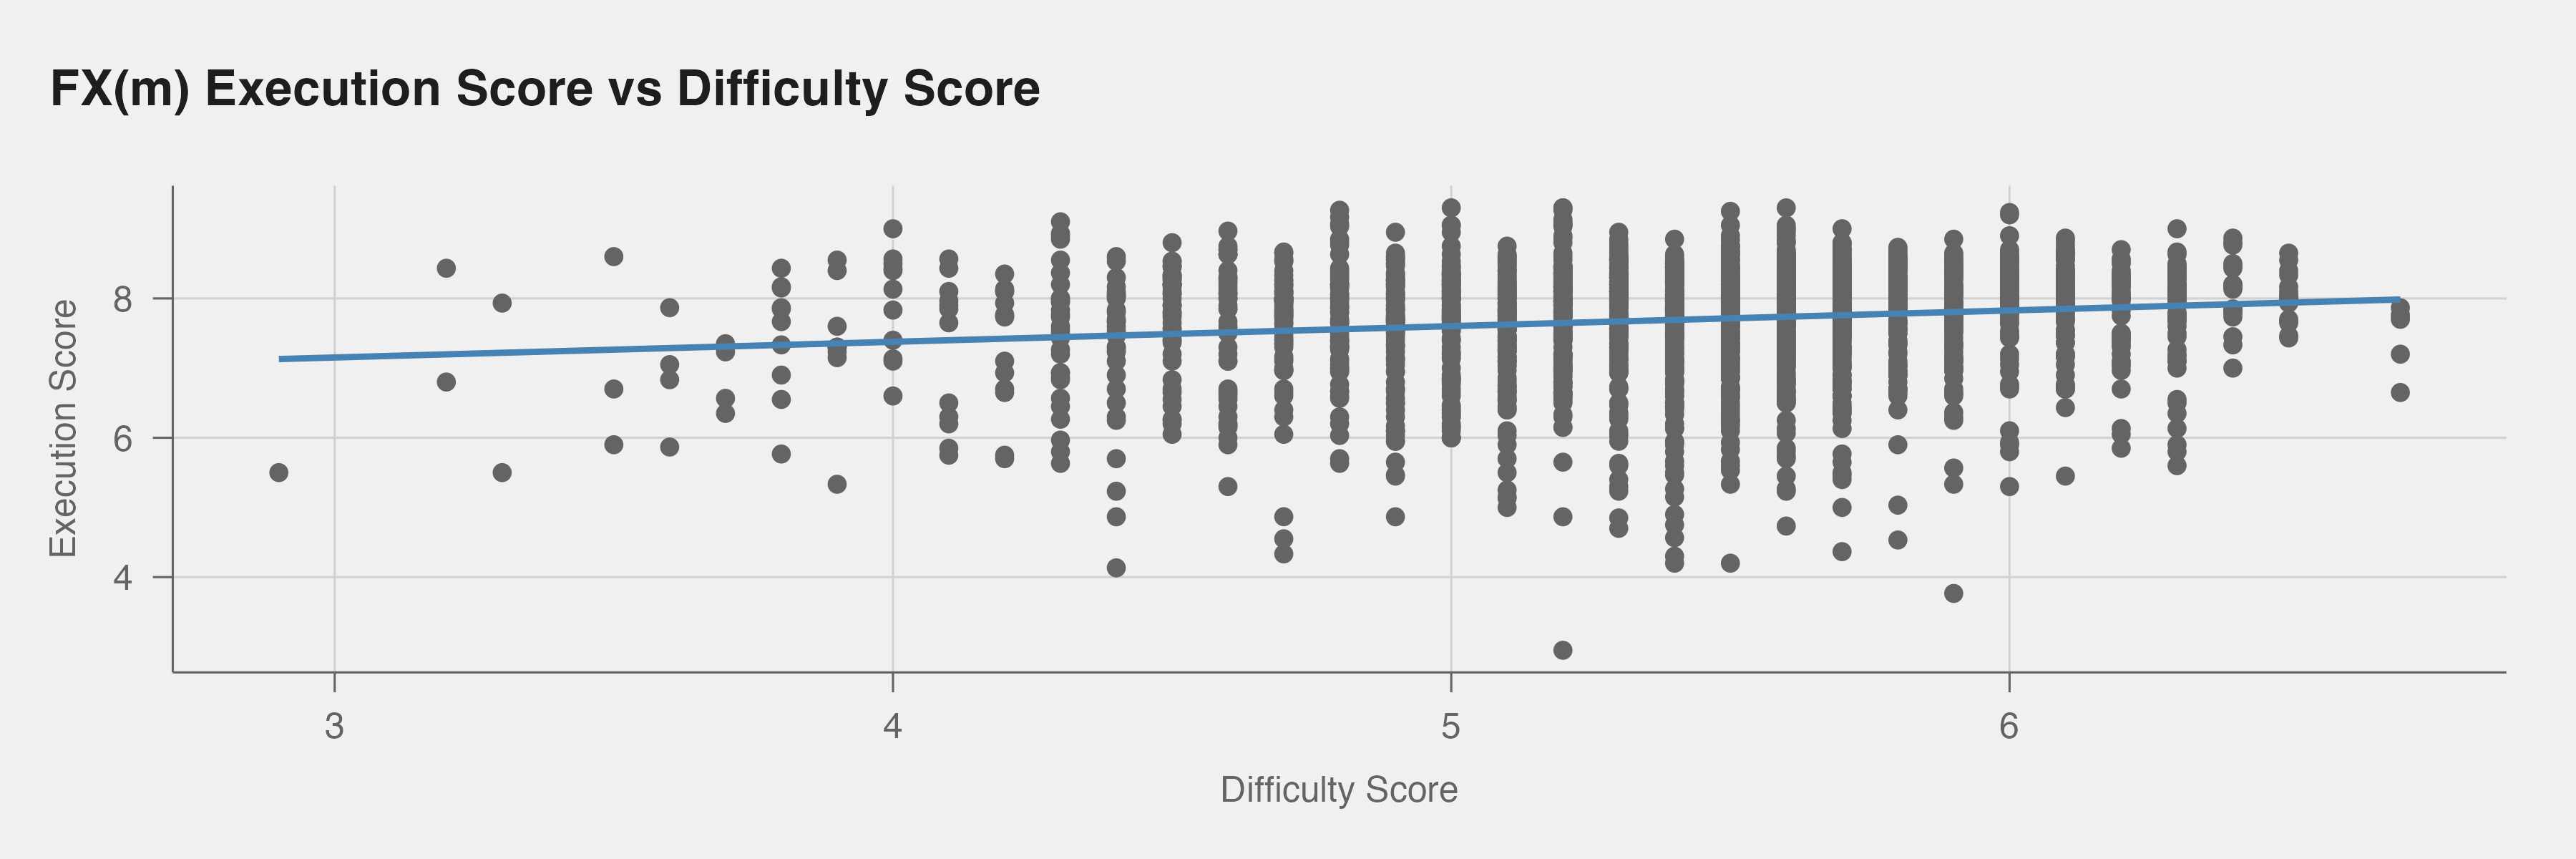
\includegraphics[width=0.7\textwidth]{../plots/fx_m_d_e.png}
   \caption{Execution Score vs Difficulty Score for FX (men)}
   \label{fig:fx_m}
\end{figure}

\subsubsection{Independence}
The independence assumption is the easiest to verify. Since the data is collected 
from different athletes, we can assume that the observations of data from different athletes are independent of each other. 
Observations from the same gymnast are not independent, but the model accounts for this by using the gymnast's name as a feature.

\subsubsection{Homoscedasticity}
\begin{figure}[H]
    \centering
    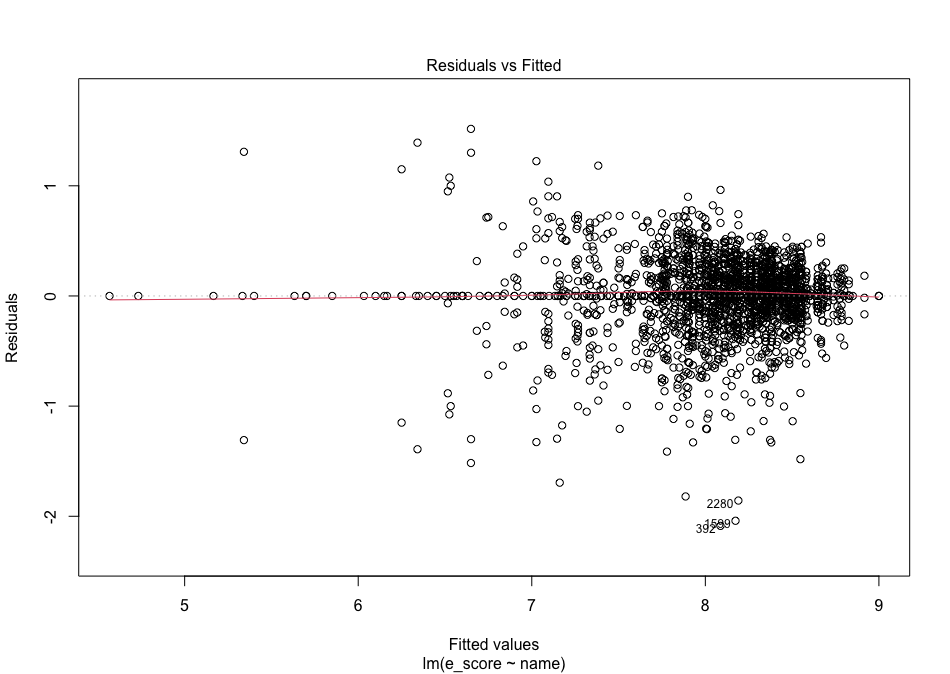
\includegraphics[width=0.8\textwidth]{../plots/m_resid_sr.png}
    \caption{Residuals vs. Fitted for Still Rings (men)}
    \label{fig:sr_m_resid}
\end{figure}

\noindent The residuals vs. fitted plot in Figure \ref{fig:sr_m_resid} shows that the residuals 
are roughly spread equally around the horizontal line without forming any discernible pattern. 
We conclude that the homoscedasticity assumption is satisfied.

\subsubsection{Normality}
We plot the distribution of \texttt{e\_score} at different levels of \texttt{d\_score}.
We see that the distribution of \texttt{e\_score} is approximately normal, albeit 
left-skewed, for the majority of \texttt{d\_score} values. For outlier values, 
the distribution of \texttt{e\_score} does not conform to the normality assumption. 
However, since these values are outliers and infrequent, we proceed with the assumption
that the distribution of \texttt{e\_score} is normal for a fixed value of \texttt{d\_score}.
Figures \ref{fig:fx_m_norm} and \ref{fig:ph_m_norm} show the distribution of \texttt{e\_score} 
for VT (women) and PH (men), respectively.
\begin{figure}[H]
    \centering
    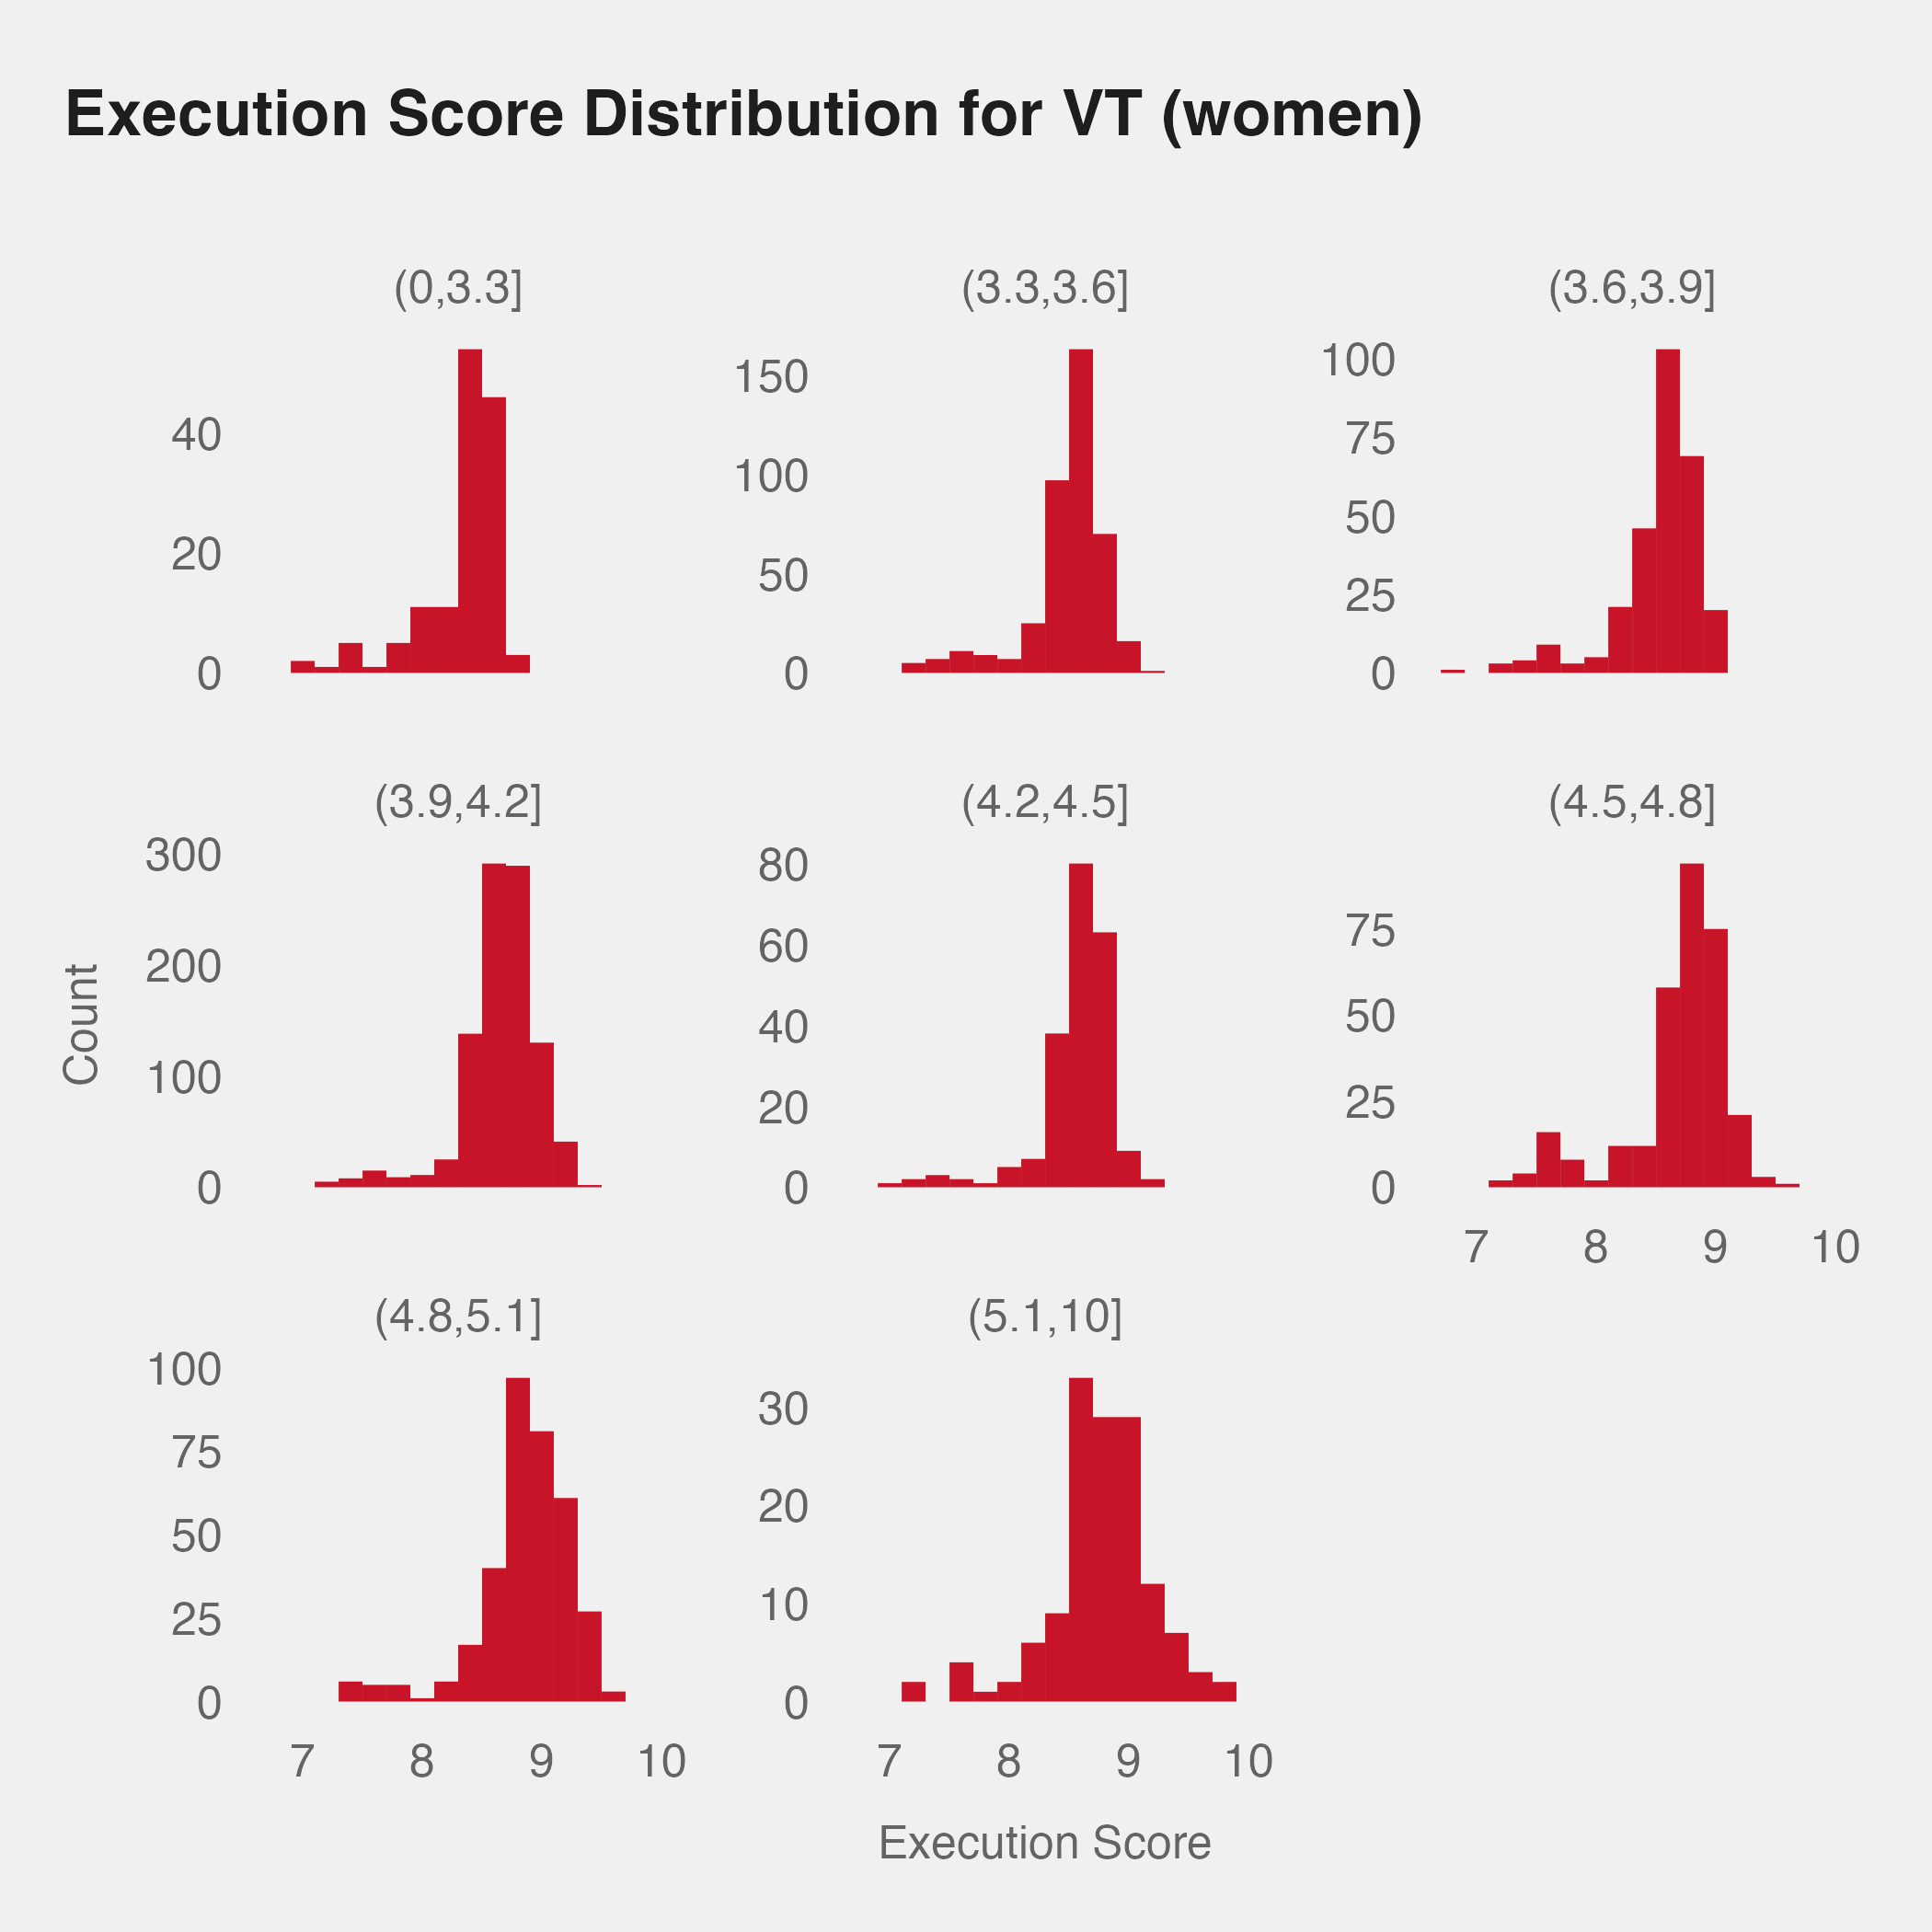
\includegraphics[width=0.6\textwidth]{../plots//w_VT.png}
    \caption{Distribution of \texttt{e\_score} for VT (women) for different bins of \texttt{d\_score}.}
    \label{fig:fx_m_norm}
\end{figure}

\begin{figure}[H]
    \centering
    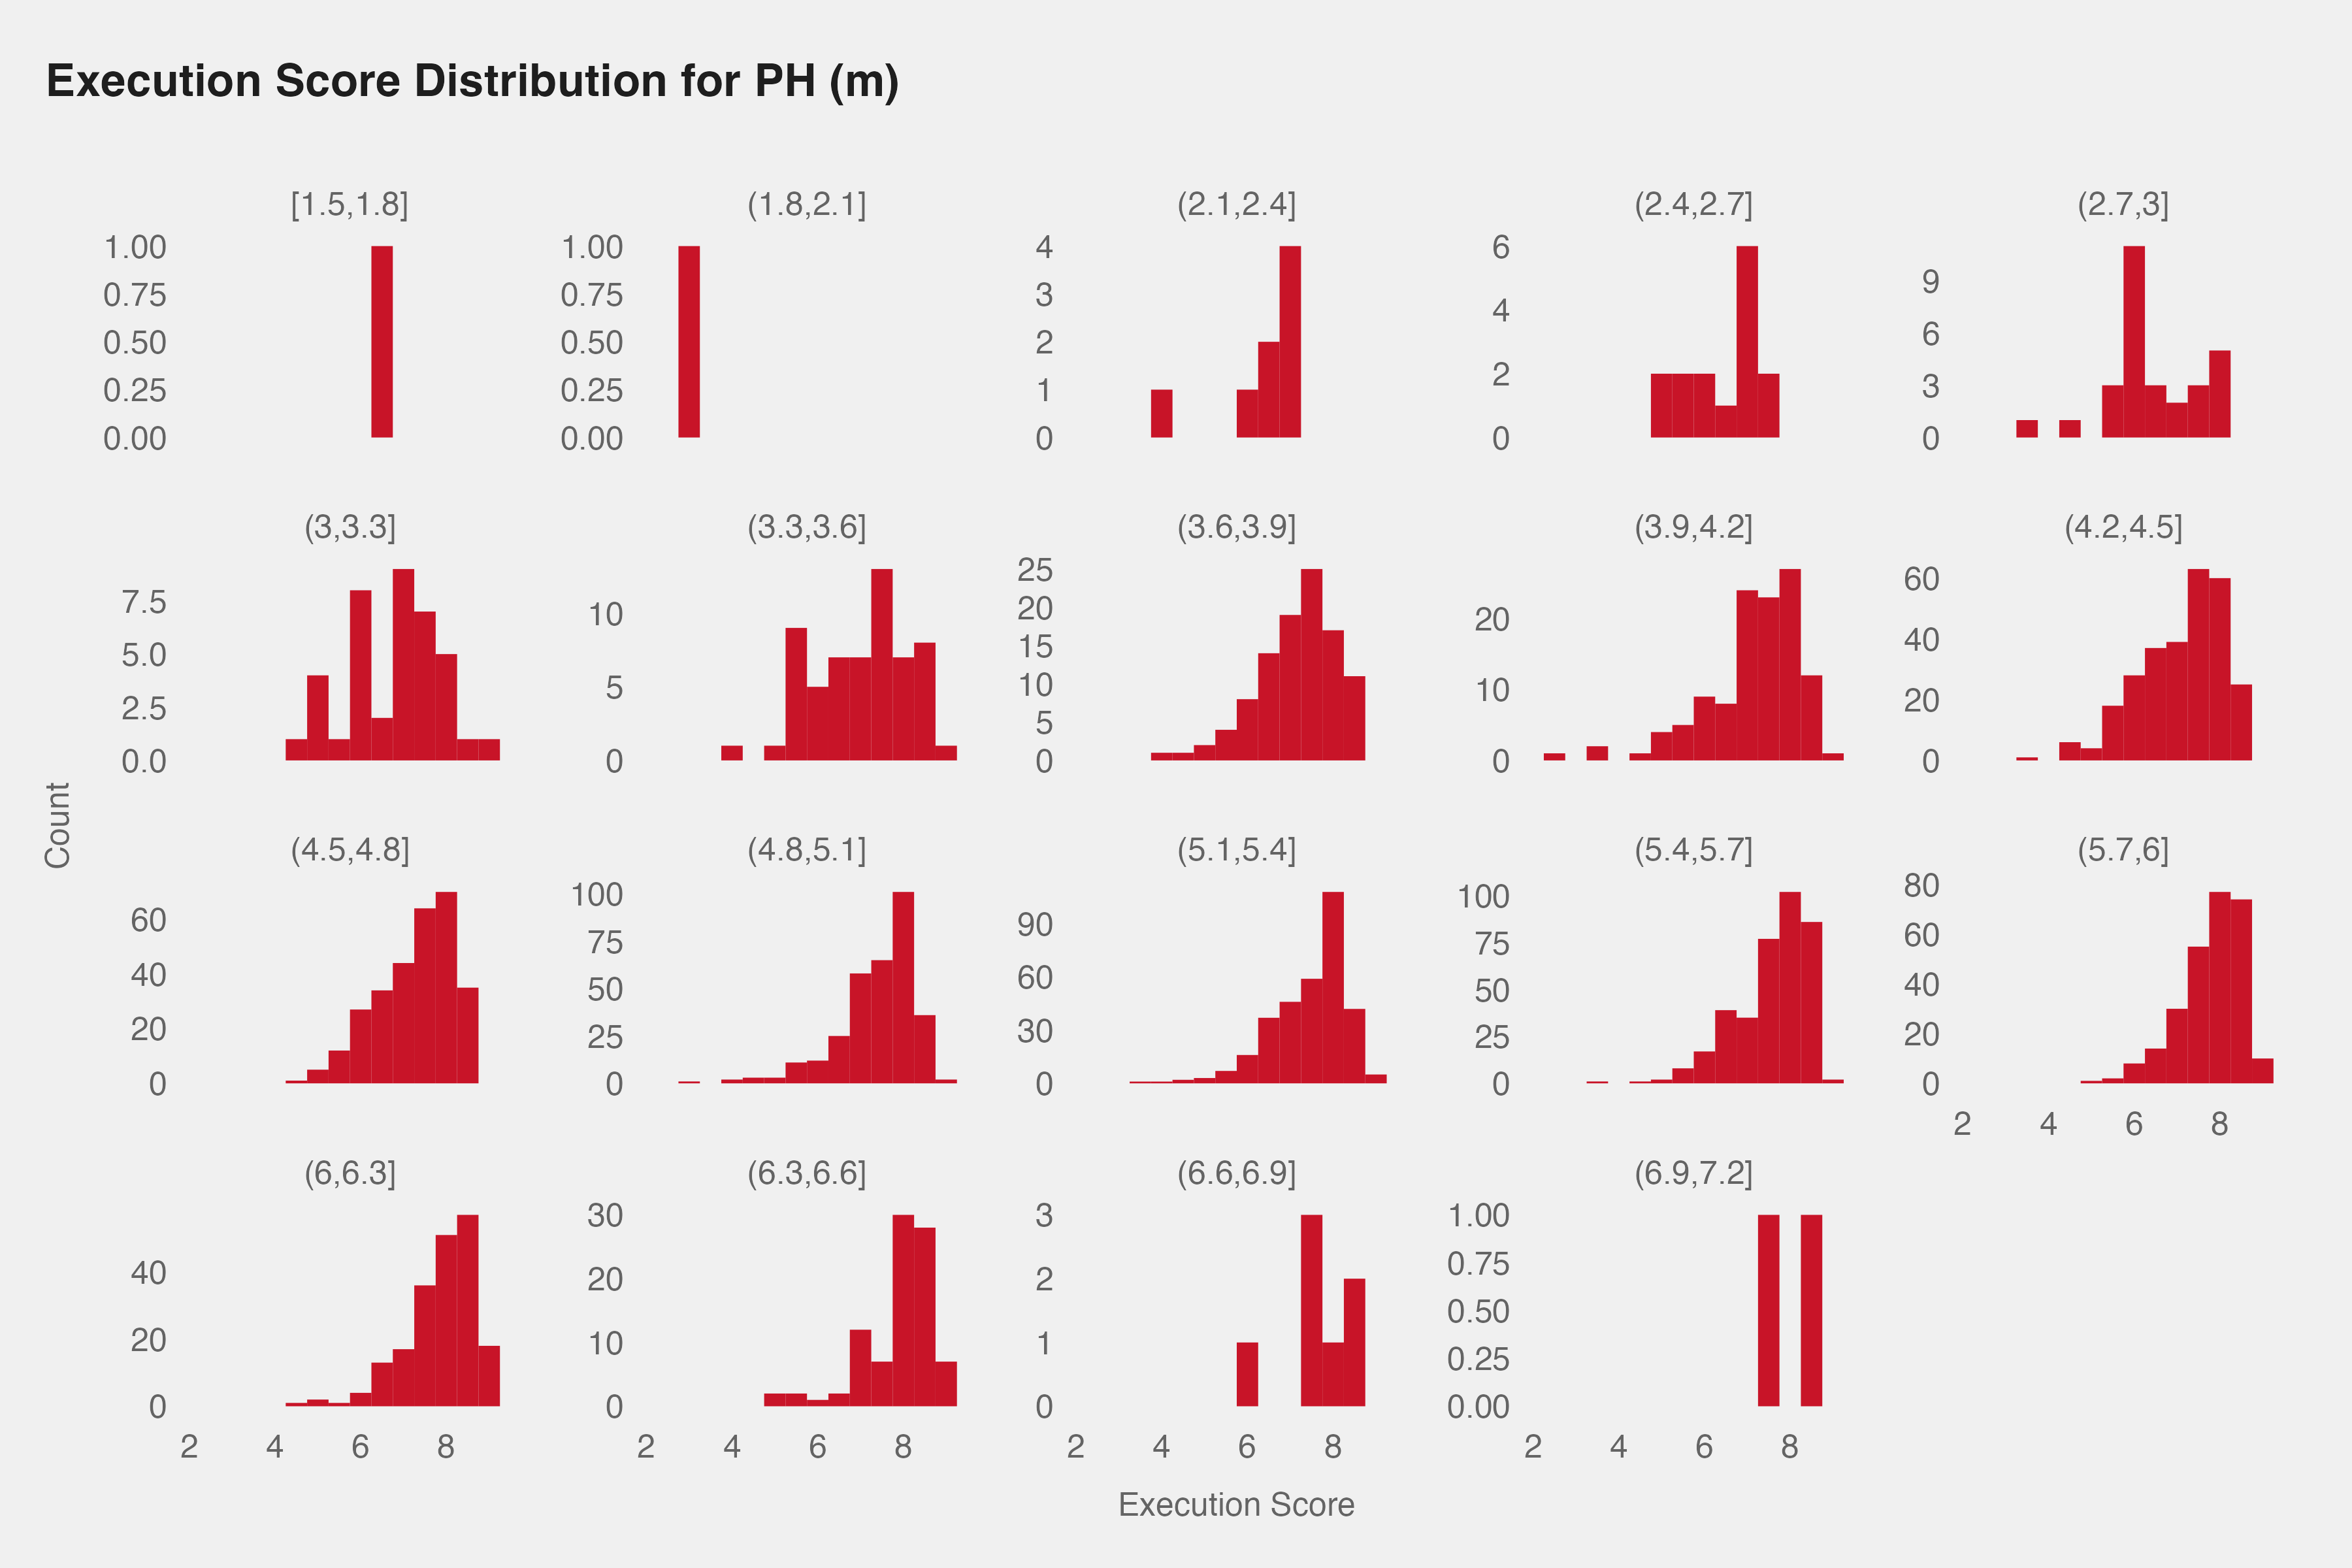
\includegraphics[width=0.6\textwidth]{../plots//m_PH.png}
    \caption{Distribution of \texttt{e\_score} for PH (men) for different bins of \texttt{d\_score}}.
    \label{fig:ph_m_norm}
\end{figure}

\subsection{Date Cleanup}
The data was found to be malformed in several ways. First, there were many repeated 
names in the data with slight variations. That coupled with incorrect country codes 
and multiple countries associated to the same athlete forced us to clean the data. 
All athlete names were deduplicated, and the country codes were corrected. 
Athletes with multiple countries were assigned the country with the most occurrences, 
except for athletes from Northern Ireland, which were forced to be part of NIR rather 
than GBR. Moreover, the data columns and values were made uniform, e.g., all lowercase 
or uppercase. Lastly, there is infrastructure in place to quickly swap out the randomly 
chosen alternates for the actual qualifiers once the Olympic team is announced. For 
alternates that have been announced, they are included in future simulations. 

\section{Modeling}\label{sec:modeling}

\subsection{Model Selection}
The linear model $Y = X\beta + \epsilon$ was chosen for its simplicity and interpretability. 
The model is easy to understand and explain, which is important for a system that is
intended to be used by coaches and decision-makers. Moreover, the model is easy to
implement and computationally efficient for simulations. The exact model formula used 
was $\texttt{e\_score} \sim \texttt{d\_score} + \texttt{name}$. A different model is 
used for each apparatus-gender pair, giving us 10 models in total.

\subsubsection{Modeling Parameters}
The model parameter interpretations follow the standard linear regression model. 
For categorical features like name, the coefficient represents the expected change 
in \texttt{e\_score} when the name is `Athlete X' as opposed to `Athlete Y' (the 
reference athlete left out by the model). For numerical features like \texttt{d\_score},
the coefficient represents the expected change in \texttt{e\_score} when \texttt{d\_score} increases 
by one unit. Due to the complexity of model layouts, we do not include the model 
parameter values in this report. 

\subsubsection{Model Performance}
The model performance as measured by $R^2$ is shown in figures \ref{fig:m_r2}
and \ref{fig:w_r2}. The models explain a reasonable amount of the variance and 
have acceptable performance.

\begin{figure}[H]
    \centering
    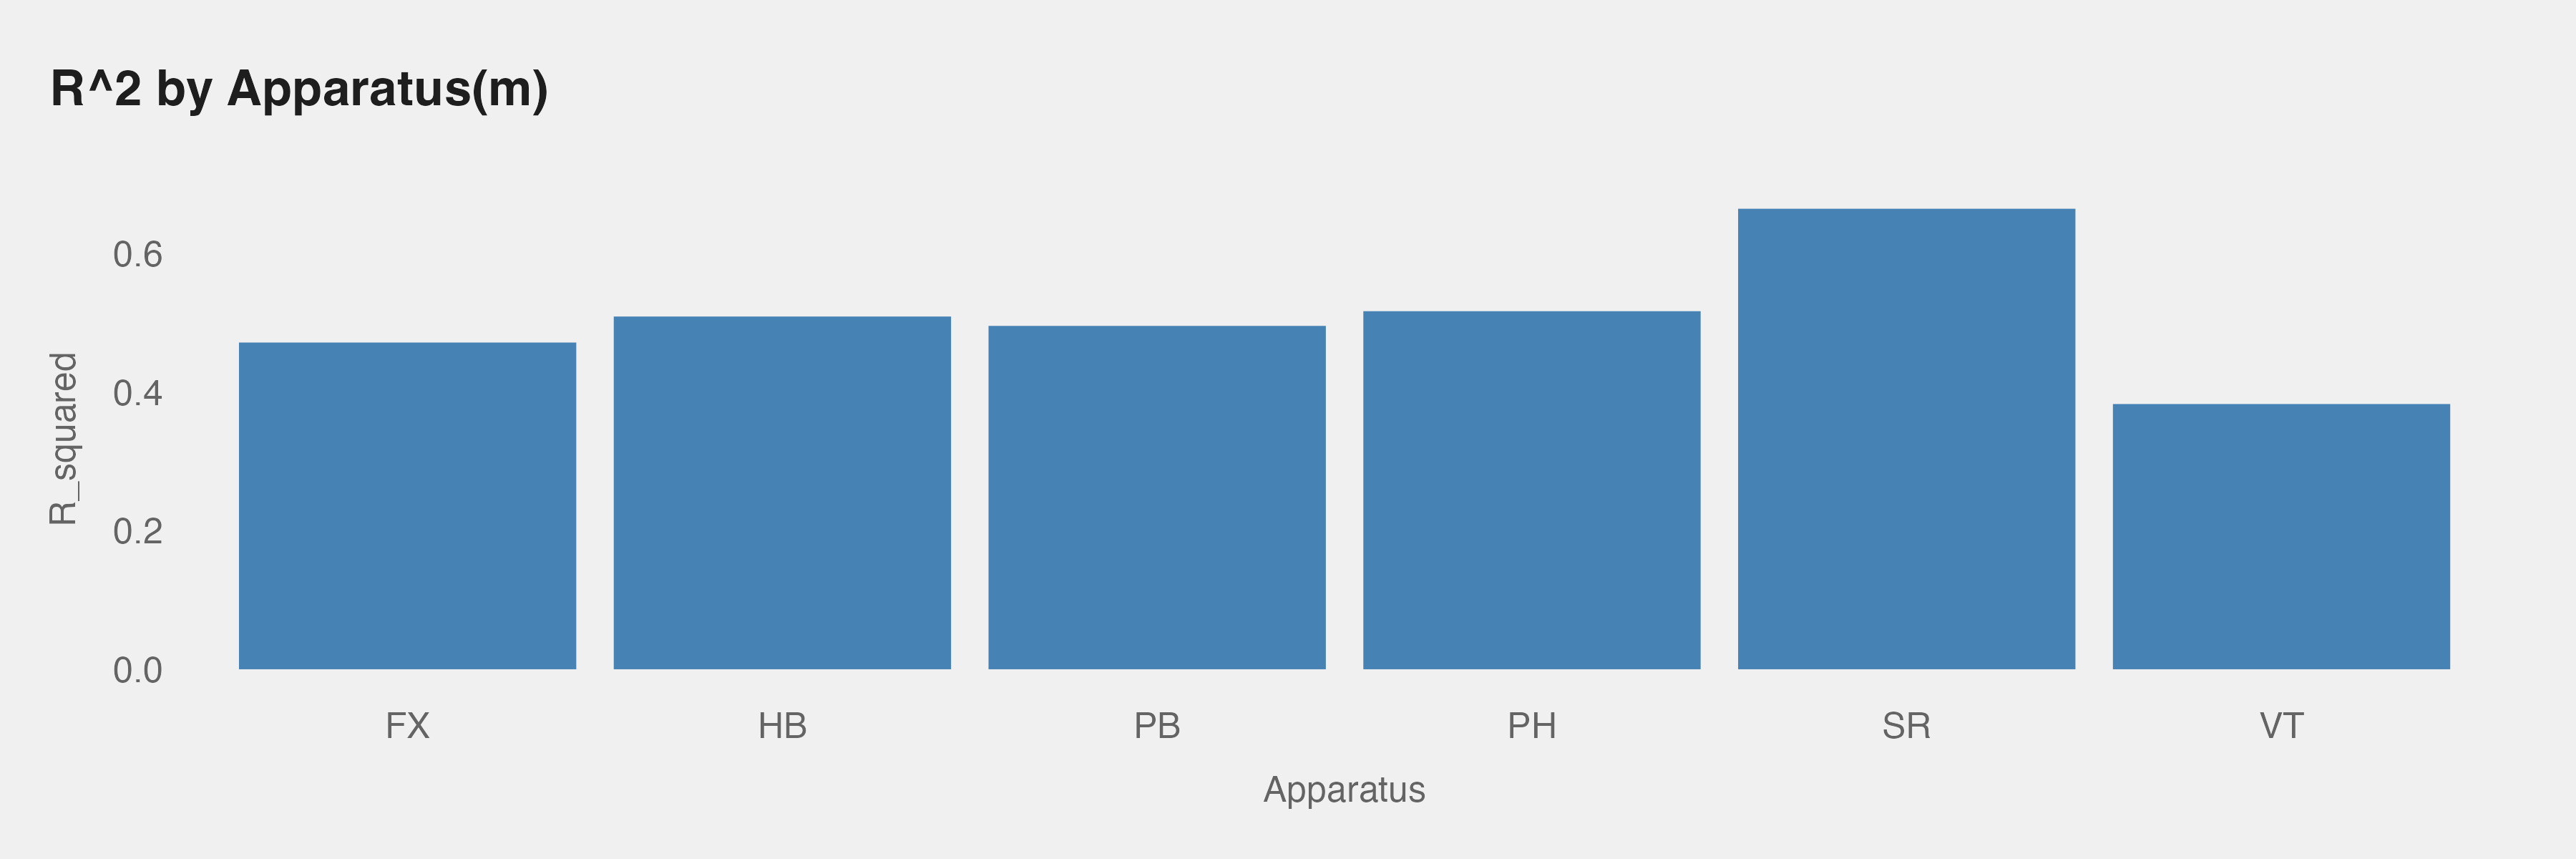
\includegraphics[width=0.8\textwidth]{../plots/m_r2.png}
    \caption{$R^2$ for FX (men)}
    \label{fig:m_r2}
\end{figure}

\begin{figure}[H]
    \centering
    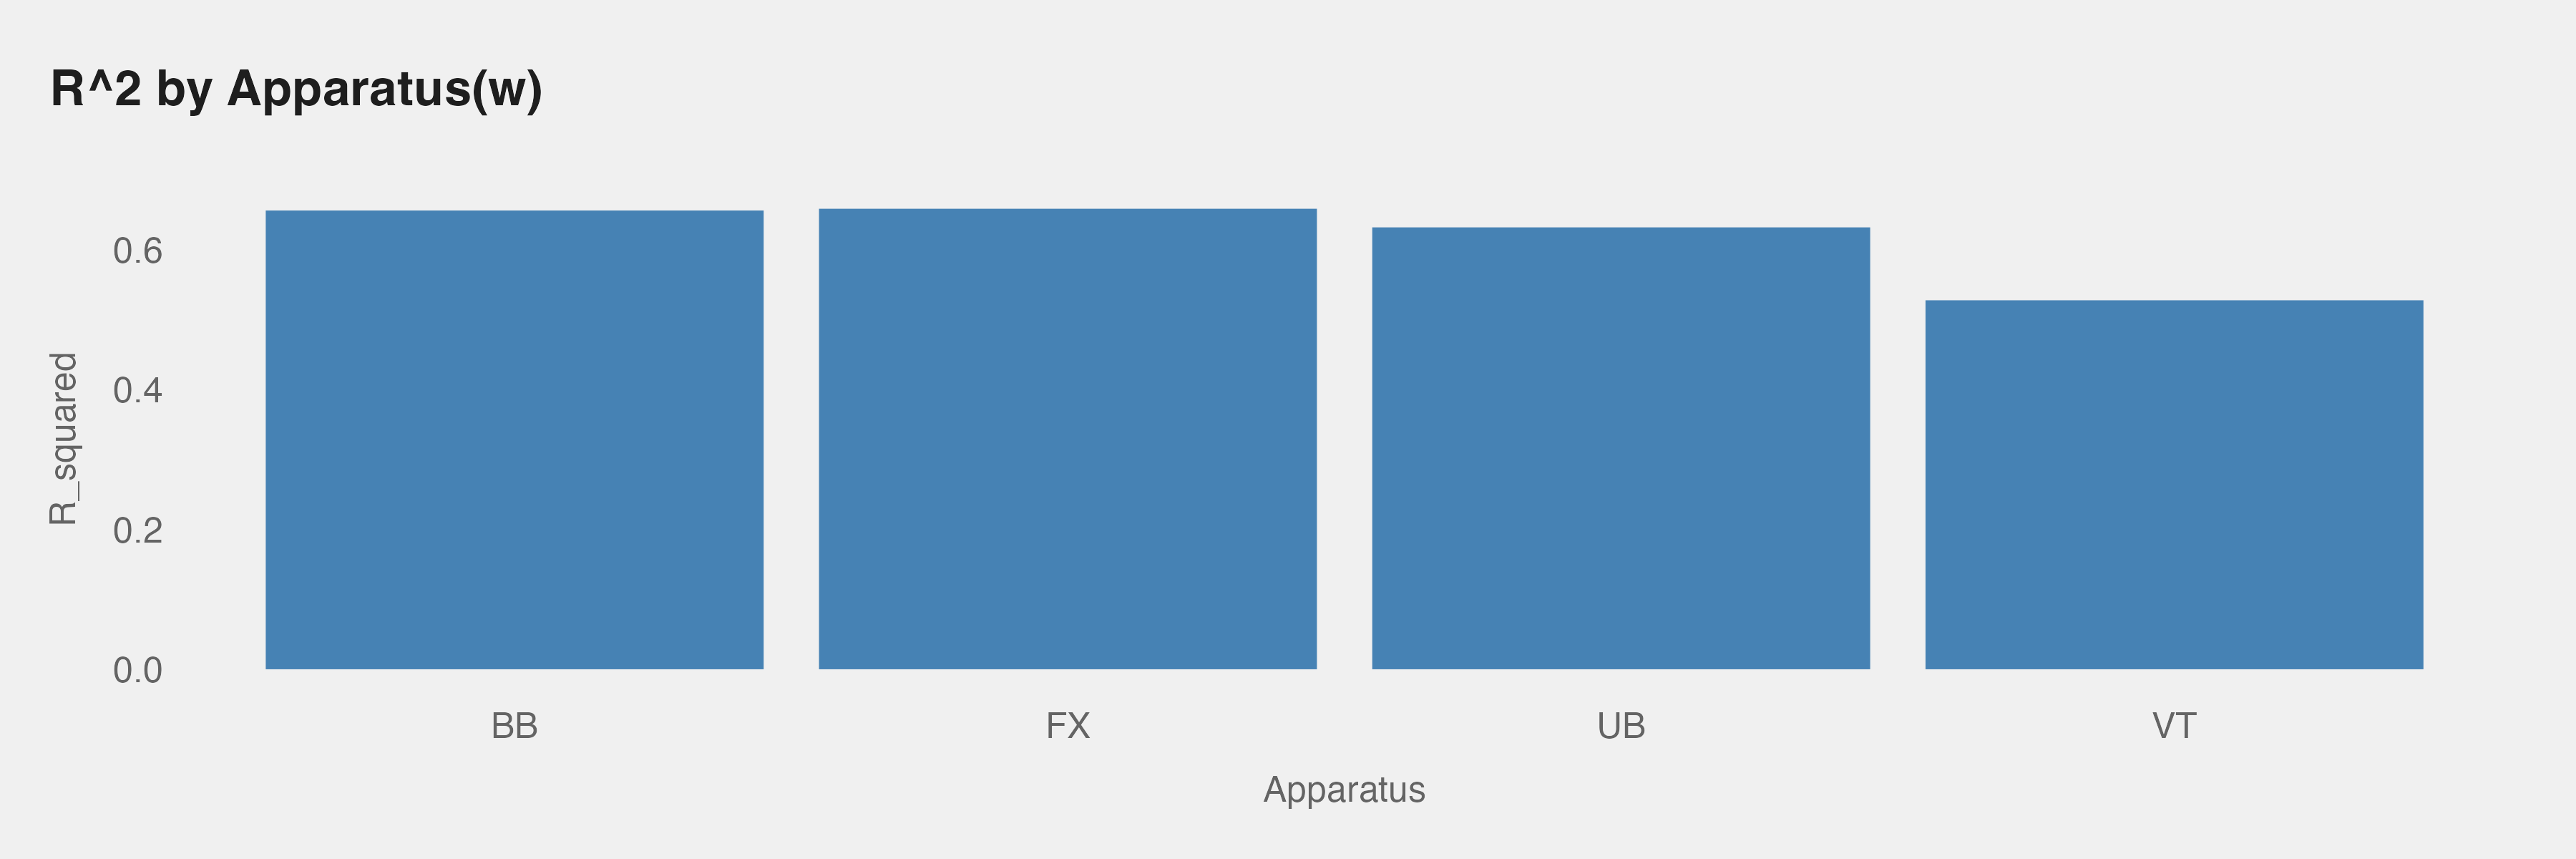
\includegraphics[width=0.8\textwidth]{../plots/w_r2.png}
    \caption{$R^2$ for FX (women)}
    \label{fig:w_r2}
\end{figure}
\noindent The best model is chosen via the AIC criterion from the \texttt{MASS} package.

\subsection{Simulations}

We explore the simulation strategy. The only fixed competitors to the competition 
are the named competitors qualifying via criterias 4-7. For the non USA qualifying teams, 
we select the top 5 all around predicted scores for a country as the team of 5. For example, 
we run one round of our model for each country, and then sum up the predicted scores 
for each individual across all apparatuses. The top 5 for that country are selected to 
be the team of 5 for that country. The top 5 for team USA is omitted as this 
is controlled via the simulations.

\ 

\noindent There are three levels to simulations: team USA assignment, apparatus allocations, and number of simulations to run. 
For each team of 5 for team USA, we randomly assign groups of 4 to each apparatus for each country. For these fixed allocations, 
we run multiple simulations to obtain a medal count distribution. The medal count is determined according to the Olympic rules for progression 
in the competition. For example, the top 8 teams in the team all around competition advance to the team finals. The top 24 
individuals in the individual all around competition advance to the individual all around finals, with a maximum of two per country, etc.

\section{System Architecture}\label{sec:system}
This application follows the three-tier architecture. That is, there is a client
application that acts only as a view layer that does not contain any direct database calls.
The client communicates with the server through a forms interface, and the server
in turn communicates with a database system to access data. More details on 
the system architecture are given in the repository README files.

\subsection{Server \& Database}

The server and database are both implemented in R. The server is a Plumber API that is run via RStudio's \texttt{plumber} package, 
while the database is a sequence of RDS files loaded by the API on startup. For more details on the server and R code,
see the repository's server README file.

\subsubsection{Server}

The server is a Plumber API that is run via RStudio's \texttt{plumber} package. 
It is responsible for handling requests from the client and returning the appropriate 
response. In particular, the server is able to explore simulations run offline 
as well as run new simulations in real time.

\subsubsection{Database}

The `database' is a sequence of RDS files loaded by the API on startup. The 
RDS files are structured as one to many relationships, where each file contains
relevant simulation data. The database files are created by following the server's 
README file.

\subsection{Client Application}

The client application consists of two pages: the simulation runner and the simulation 
explorer. The simulation runner allows the user to run new simulations and view the
results. The simulation explorer allows the user to explore simulations that have
already been run. We developed a simple user interface that allows the user to
select a team of 5, allocate them to apparatuses, and run simulations. The results 
are displayed in the form of bar charts, showing the medal count for each team 
or individual through the simulations.

\subsubsection{Simulation Runner}

\begin{figure}[H]
    \centering
    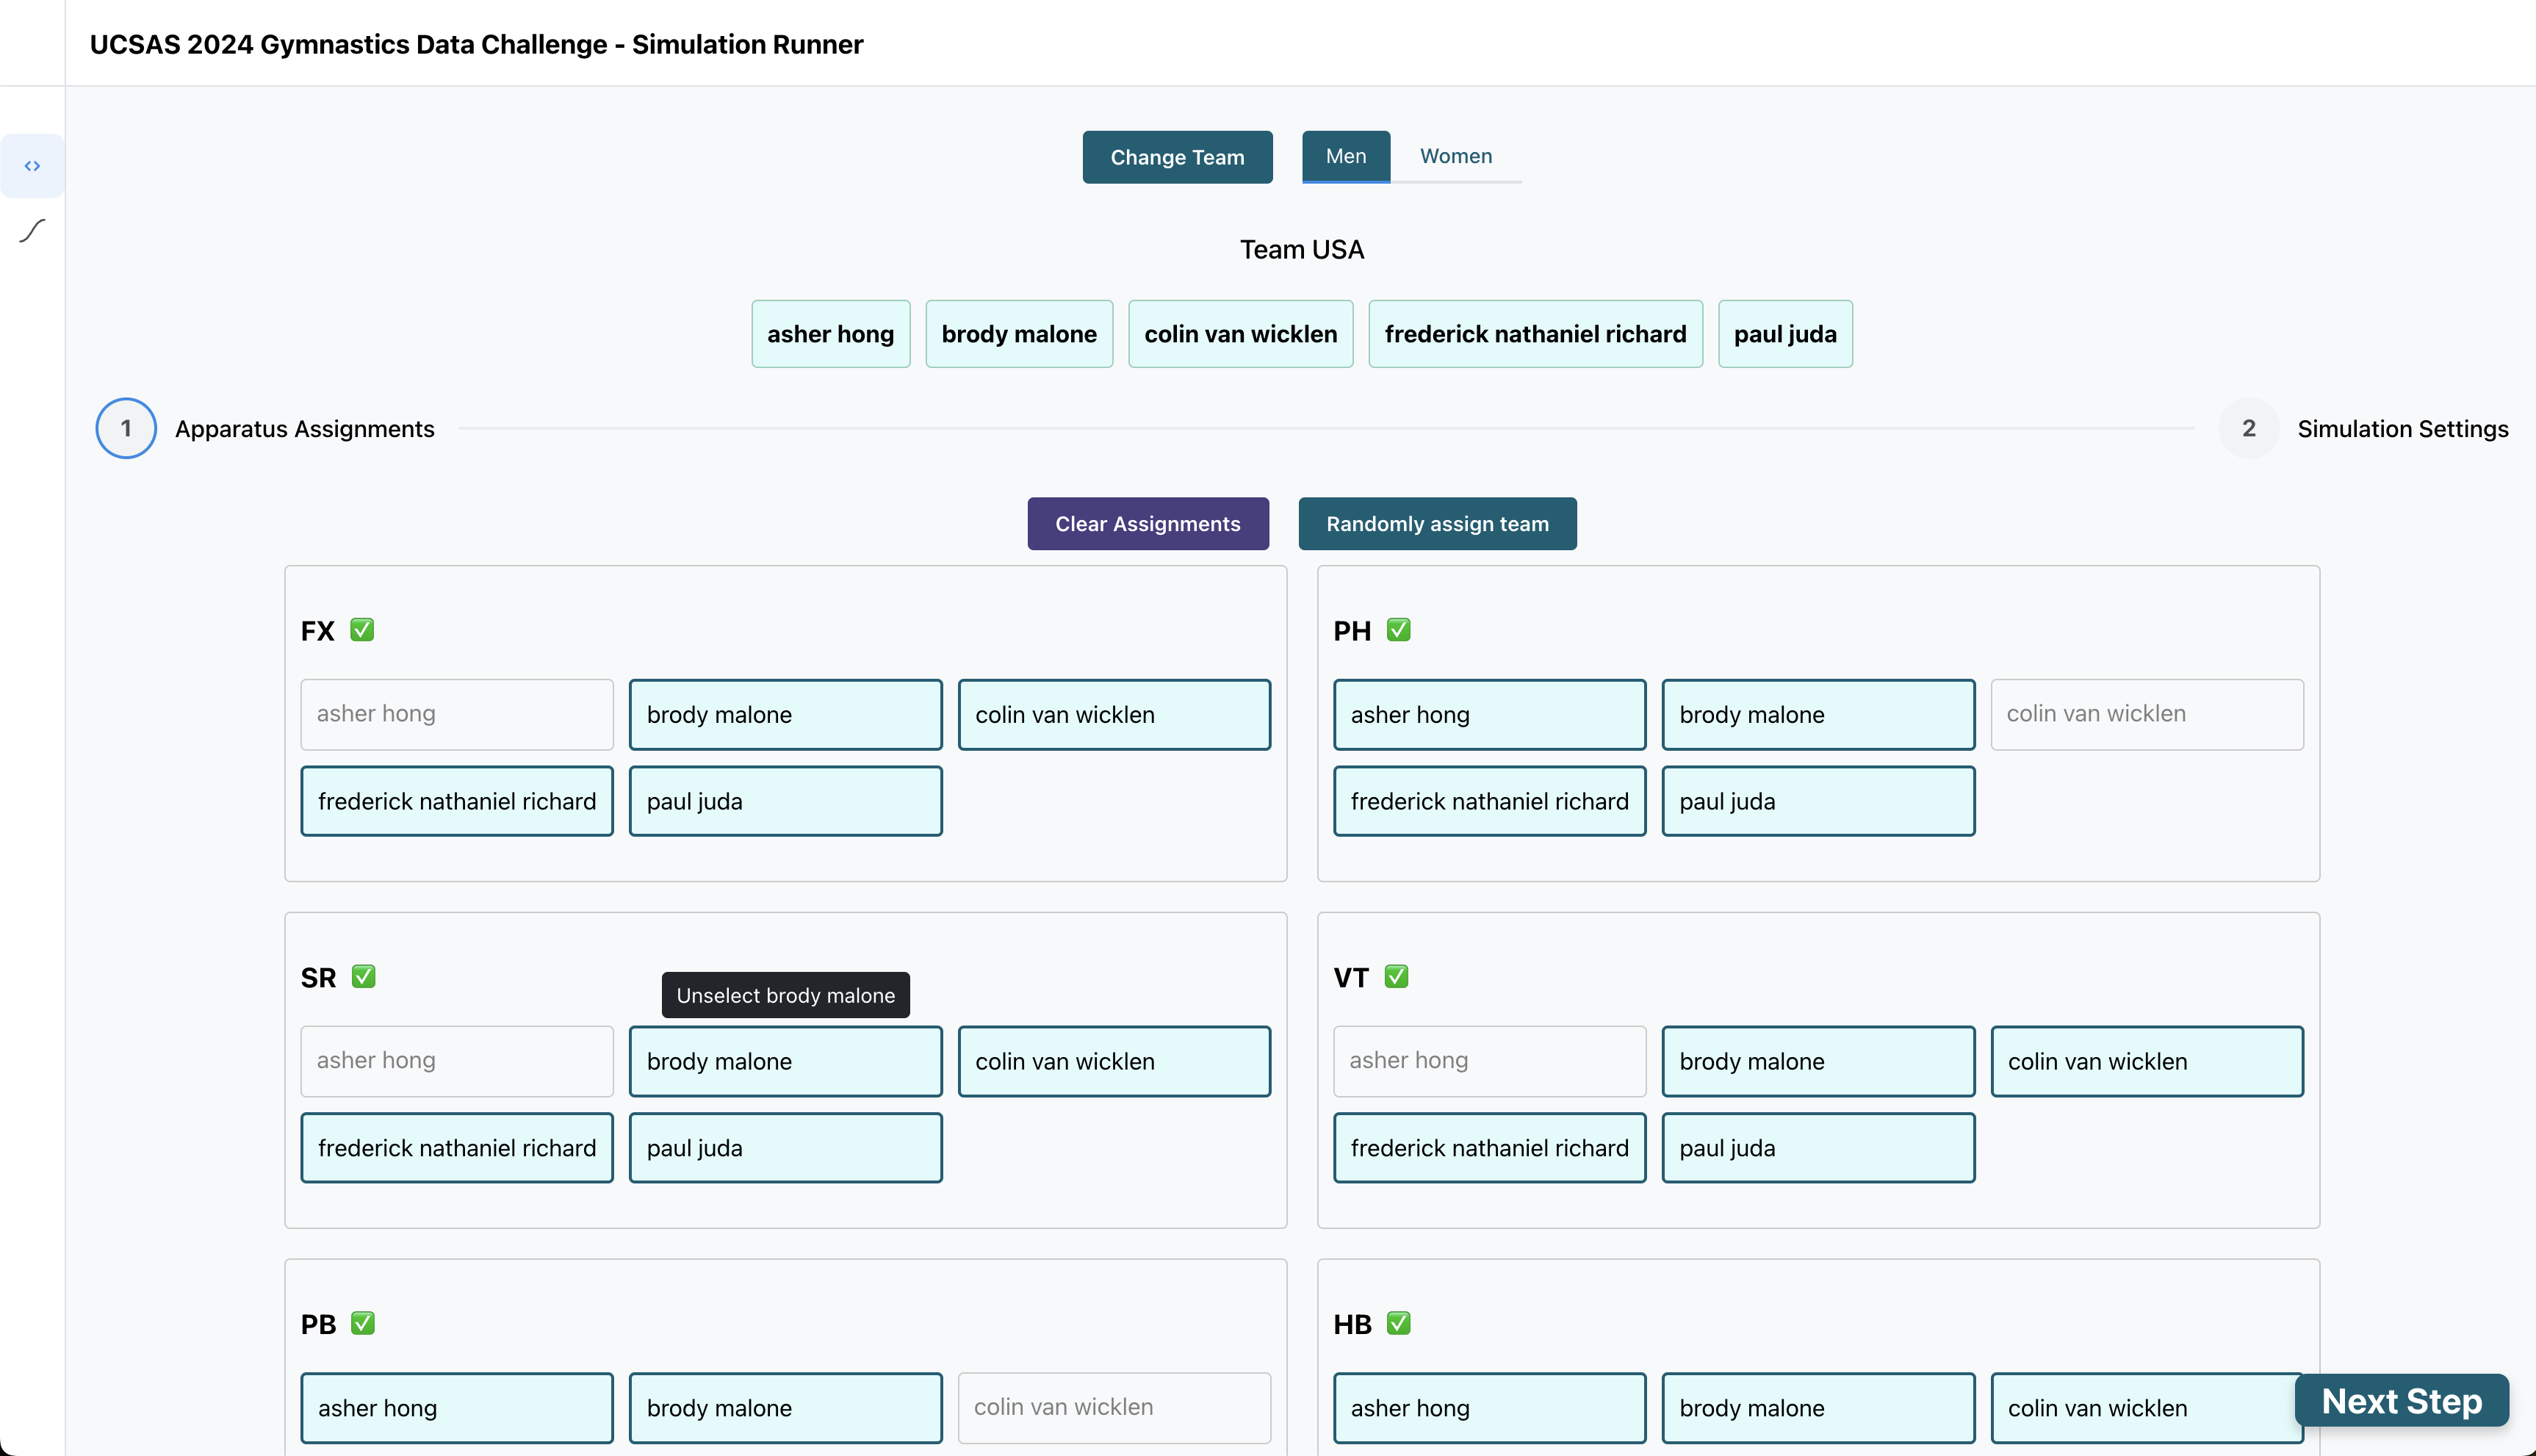
\includegraphics[width=0.8\textwidth]{./simulation_runner.png}
    \caption{Simulation Runner Apparatus Allocations}
    \label{fig:sim_runner}
\end{figure}

The simulation runner, shown in Figure \ref{fig:sim_runner}, allows the user to select a gender and associated team of 5, 
from which they allocate to apparatuses. The user is able to do the assignments manually or pick 
one at random. There are a variety of UI features that prevent the user from picking a bad team, 
e.g., an apparatus allocation is only possible for users that have data points for that apparatus. 
If no valid team is assignable, the user is notified. Once a valid team is selected, the user 
sees results as in Figure \ref{fig:sim_results}. A figure is shown for team all around, individual all around, and all apparatus events.

\begin{figure}[H]
    \centering
    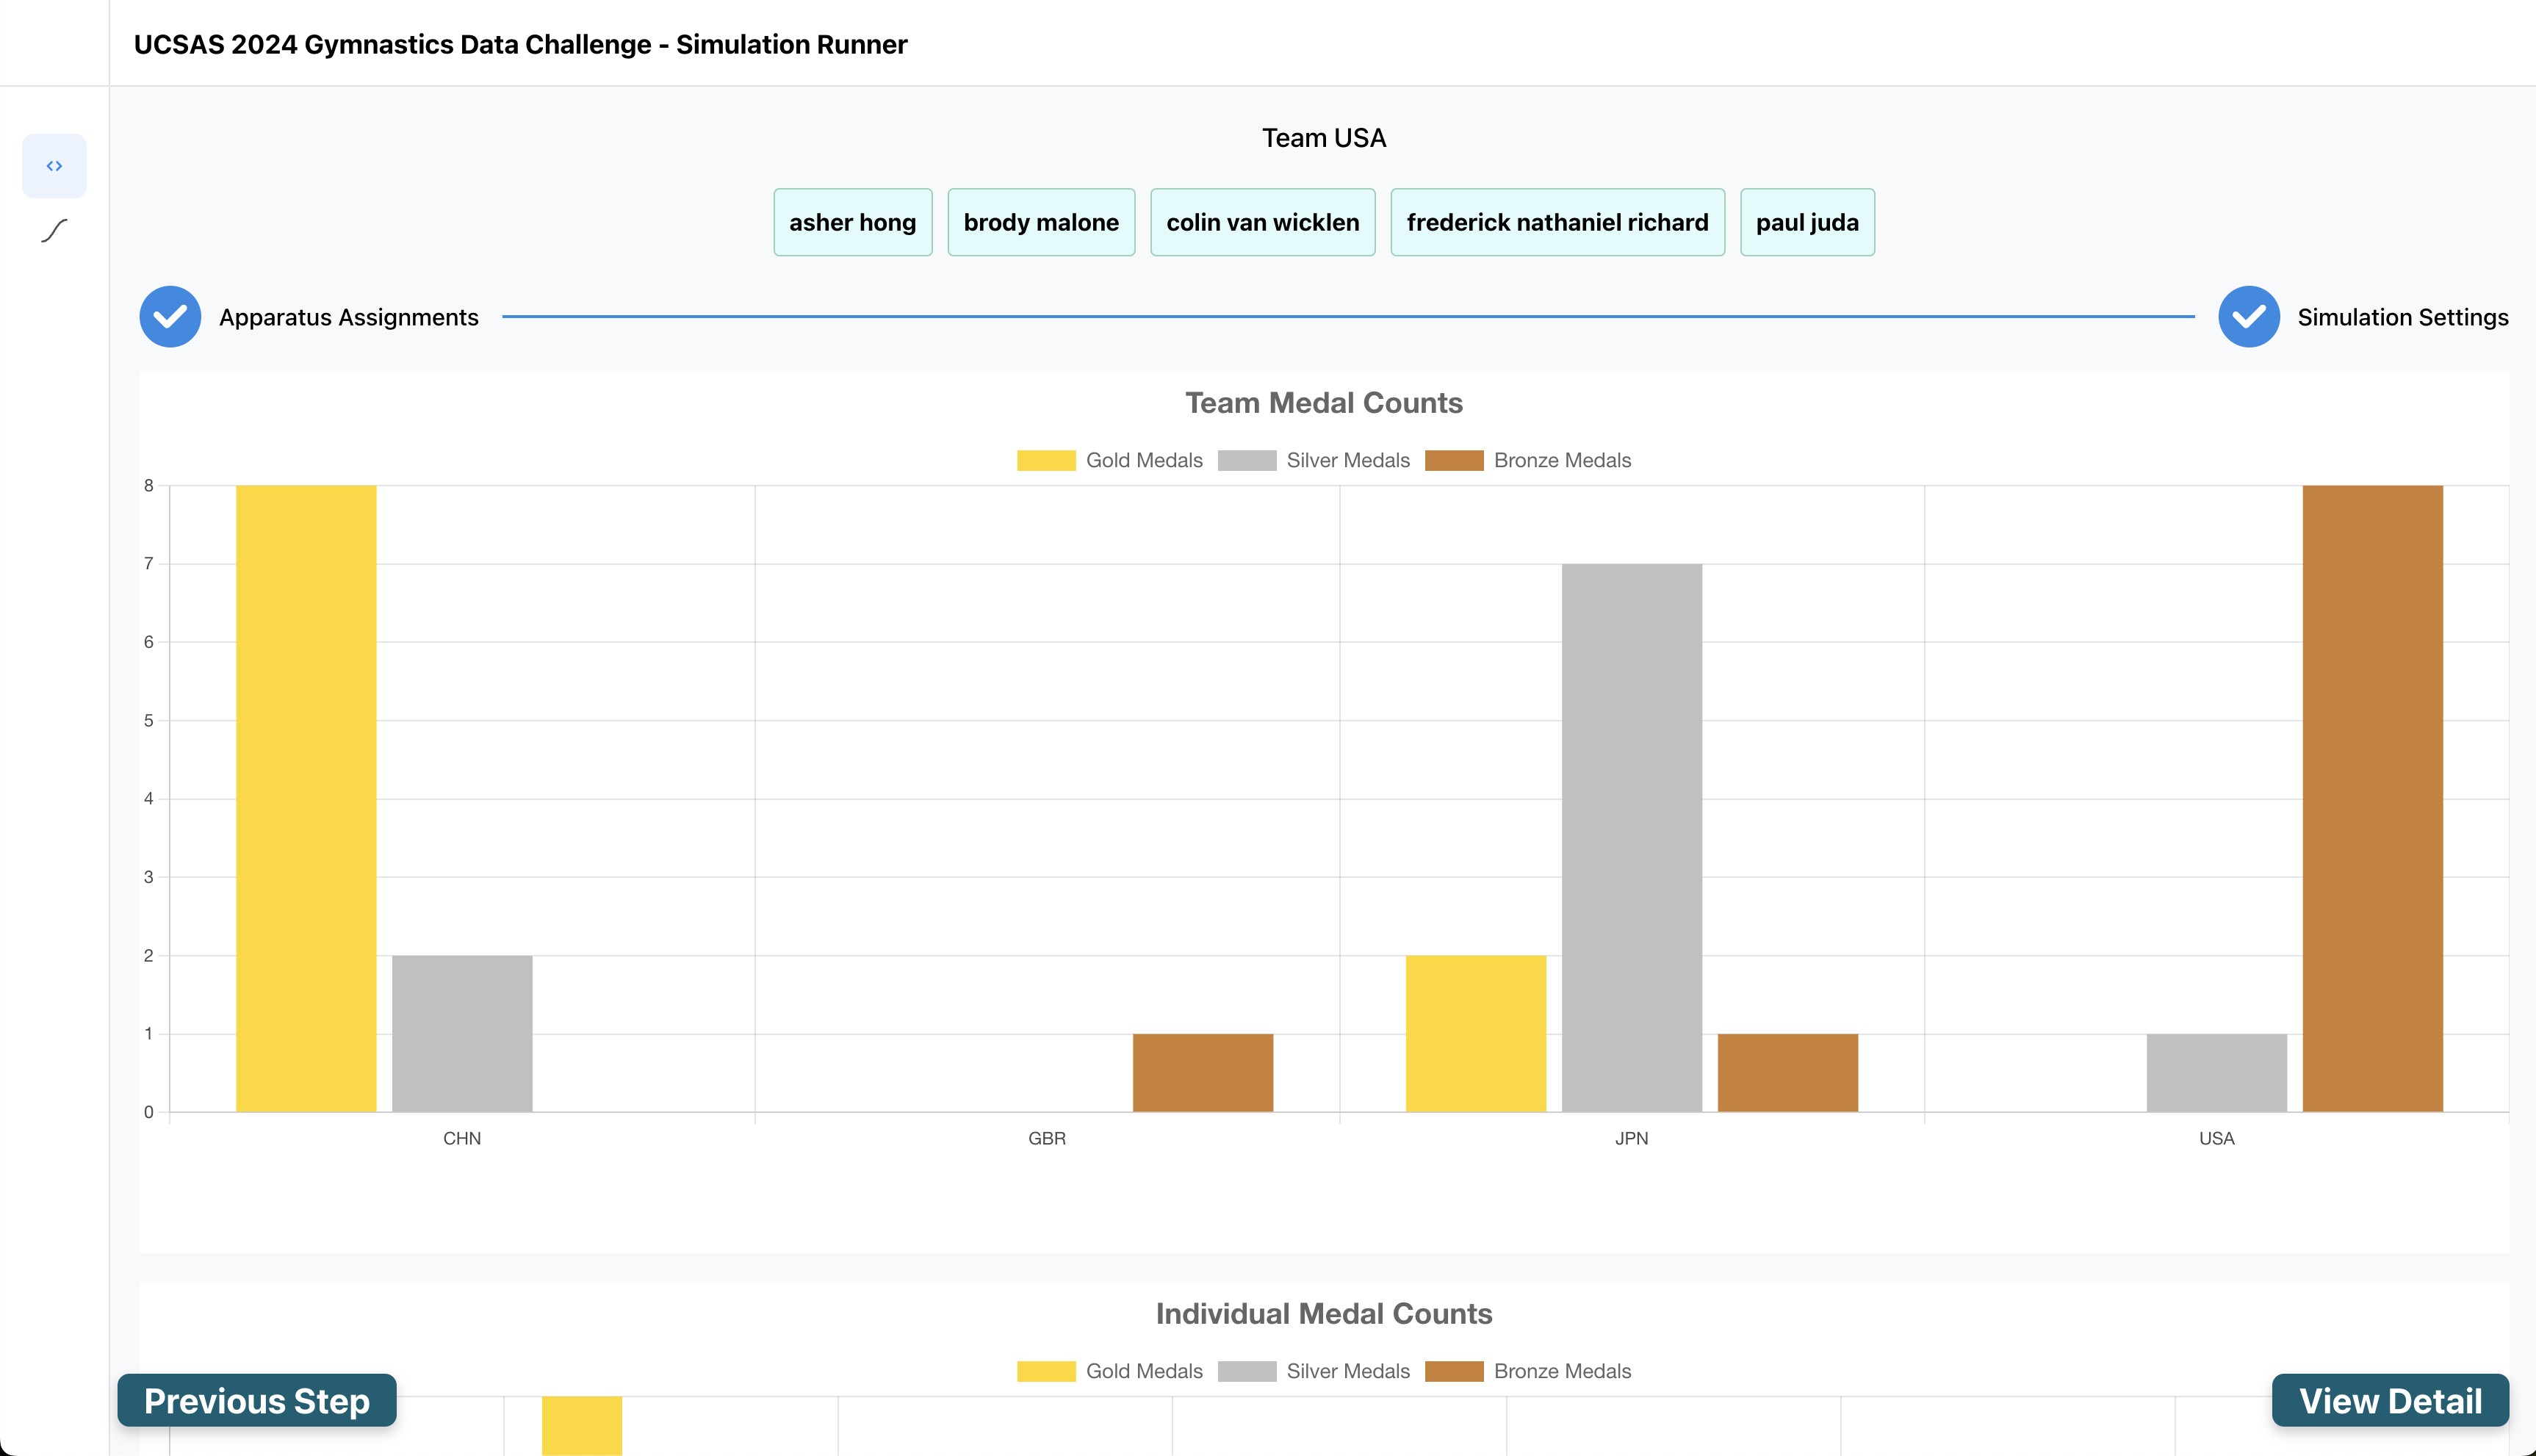
\includegraphics[width=0.8\textwidth]{./results_viewer.png}
    \caption{Simulation Runner Results}
    \label{fig:sim_results}
\end{figure}

\noindent Additionally, the user is able to view the apparatus and team allocations of all 
other countries in the simulations. This allows the user to compare their team
to other teams and see how they stack up.



\subsubsection{Simulation Explorer}

The simulation explorer runs entirely similar to the simulation runner, except that the user
is able to explore simulations that have already been run via the \texttt{run\_simulations.R} script in the server. This 
process is detailed in the repository.

\subsubsection{Implications}
The system offers a data-driven approach to team selection, allowing coaches and decision-makers to make informed choices. 
The idea was not to provide recommendations, it was to provide a tool to non data scientists to let them answer 
their own questions. The user experience is designed to be simple and intuitive, allowing for easy exploration of
different team compositions and outcomes. The choice of bar charts for the results was intentional, as it allows
for easy comparison of different teams and individuals across a variety of simulation.
\end{document}
